Table~\ref{table-spkshow-perf} shows the average $Fm$ related to $SpkShow$ for the different systems, and for the oracle system which is made of the best system for each $SpkShow$.
\begin{table}[t]
\begin{center}
\footnotesize
\begin{tabular}{r||c|c|c|c}
						& PERCOL 				&	 QCOMPERE 			& SODA 					& Oracle 				\\
\hline\hline
average $Fm$ 			& 36.1 	 				& 38.1 					& 35.1 					& 46.2	 				\\
\hline
average $Fm$ for 		& \multirow{2}{*}{62.8}	& \multirow{2}{*}{68.4}	& \multirow{2}{*}{61.9}	& \multirow{2}{*}{72.2}	\\
in dict. $SpkShow$ 		&  						&  						&  						& 						\\
\hline
\#$SpkShow$ out 			& \multirow{2}{*}{200}	& \multirow{2}{*}{209}	& \multirow{2}{*}{204}	& \multirow{2}{*}{172}	\\
of dict. 				& 	 					& 	 					& 	 					& 						\\
\hline
\#$SpkShow$ in dict. 	& 277					& 268 					& 273 					& 305					\\
\hline
\#$SpkShow$ in dict. 	& \multirow{2}{*}{79}	& \multirow{2}{*}{63}	& \multirow{2}{*}{86} 	& \multirow{2}{*}{63}	\\
with $Fm=0$ 				& 	 					& 	 					& 	 					& 						\\
\hline
\end{tabular}
\caption{Average system performance related to $SpkShow$}
\label{table-spkshow-perf}
\end{center}
\end{table}
We can notice the large number of $SpkShow$ which are not in the dictionary of the three systems: about 40\% for each system. As they do not have any model, they obviously cannot be identified, leading to a rather poor global $Fm$. More interestingly, the number of in-dictionary $SpkShow$ that are not recognised at all is not negligible: they represent between 23.5\% and 31.5\% of the in-dictionary $SpkShow$, depending on the system.

Figure~\ref{fig:FMeasureDistribution} plots the distribution of all the $SpkShow$ in the system dictionaries, according to their performance expressed in terms of $Fm$, for the different systems. We can see that the average performance (between 61.9\% and 72.2\%) is not at all representative of performance obtained for each $SpkShow$: speakers are either not recognized or well recognized. Indeed, if we compute the average performance for $SpkShow$ which have $Fm \neq 0$, the average $Fm$ grows to 87.9\% for PERCOL, 89.5\% for QCompere and 90.3\% for SODA. 

% \begin{figure}[!h]
% \includegraphics[scale=0.6]{figures/PQS-mono-model.eps}
% \caption{$spkShow$ performance distribution, for each system}
% \label{PQS}
% \end{figure}

To evaluate the impact of the automatic speaker diarization, the analysis of the speaker performance when systems rely on the reference speaker diarization is carried out. Results for PERCOL system is shown in Figure~\ref{fig:autoVSref}.  The bi-modal distribution of performance (speaker either well recognized, or not at all recognized) is dramatically emphasized with the reference diarization.
The comparison of the speaker identification performance between using the reference or automatic speaker diarization, carried out on PERCOL and SODA systems, shows that 38 $SpkShow$ (out of 277 in-dictionary speakers) for PERCOL and 14 $SpkShow$ (out of 273 in-dictionary speakers) for SODA present a null F-measure ($Fm_i=0$) with the automatic speaker diarization and a F-measure above 90\% with the reference one. For these particular $SpkShow$, the quality of the automatic speaker diarization is the main reason of the poor speaker identification performance. A fine-grained analysis of the speaker diarization outputs highlighted segment frontier errors, clustering confusion errors, or both of them. 
In addition, we considered the $SpkShow$ for which a null F-measure is obtained even with the reference diarization: 41 for PERCOL and 72 for SODA. For half of these $SpkShow$, the amount of testing data was less than 10s. For the other half, the amount of training data could not explain the poor performance as, on average, more than 600s were available for each of those $SpkShow$.
Focusing on the 12 $SpkShow$ which have a null F-measure with reference diarization in both systems, the analysis revealed that these segments had very poor acoustic quality: a large amount of overlapped speech for 4 $SpkShow$ (from 20 to 90\% of overlapped speech according to  $SpkShow$), an entire interview made by phone for one $SpkShow$, poor sound quality with reverberation for another one, and large background noise (street, assembly background voices, applause, etc) or music for 8 of them.

\begin{figure}[t]
\centering
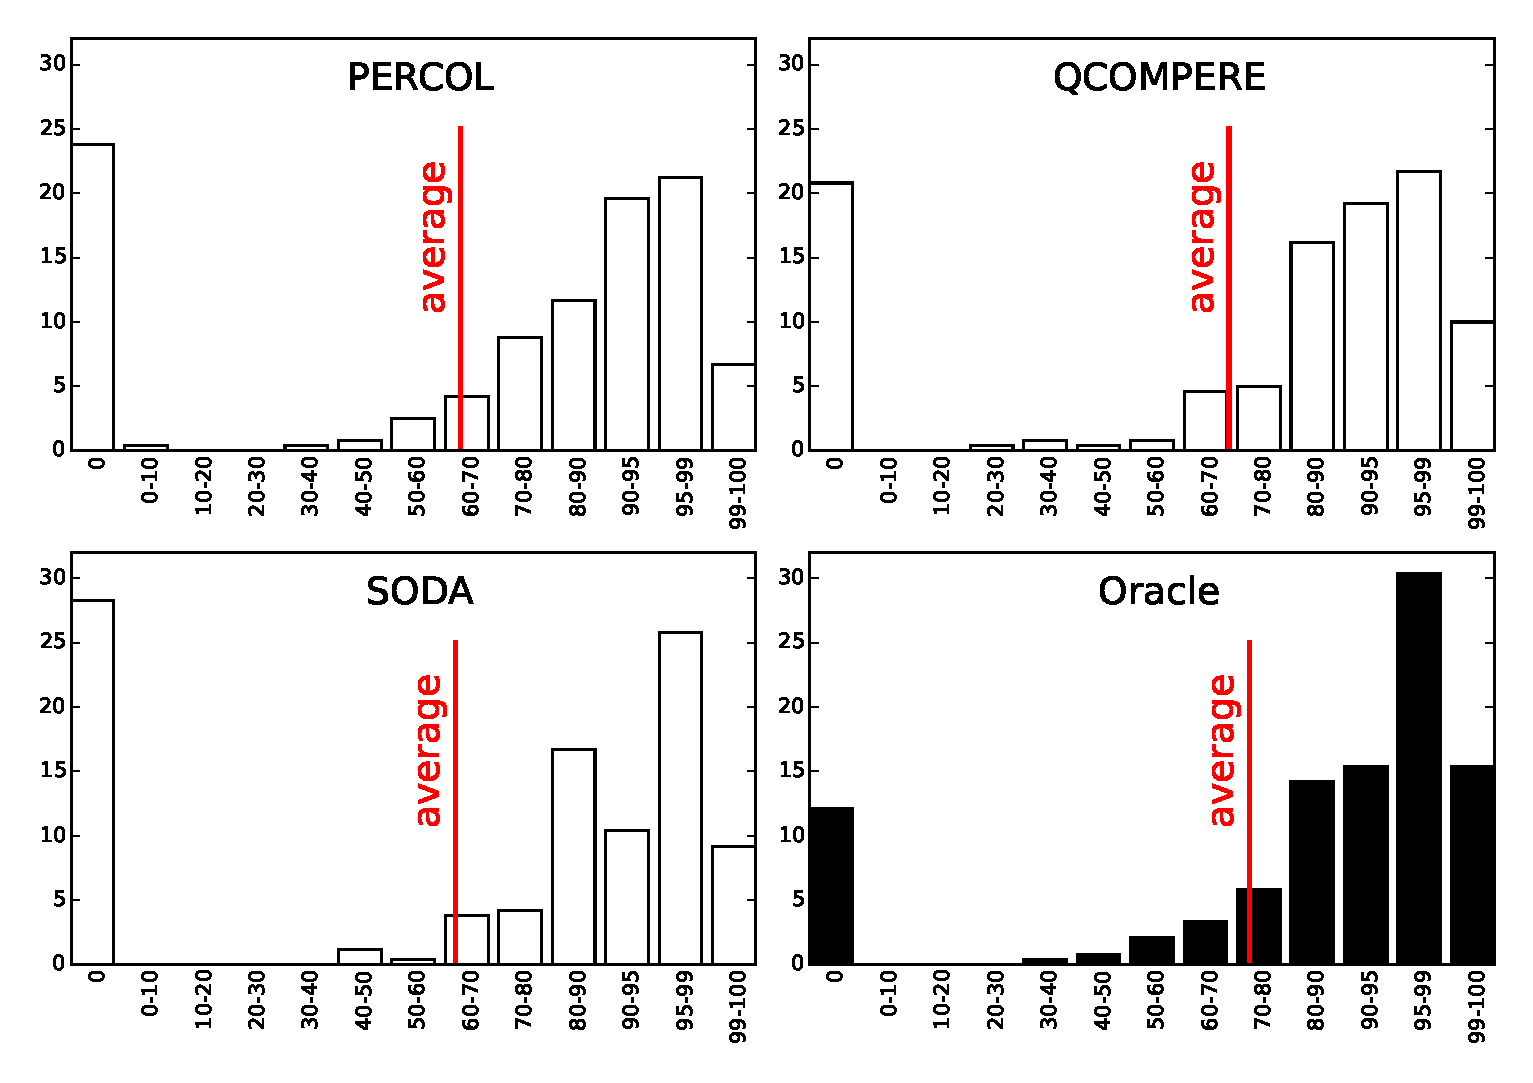
\includegraphics[width=\linewidth]{figures/bimodal.eps}
\caption{Distribution of $SpkShow$ according to system performance expressed in terms of $Fm$}
\label{fig:FMeasureDistribution}
\end{figure}


\begin{figure}[t]
\centering
\includegraphics[width=\linewidth]{figures/ref.eps}
\caption{Effect of diarization errors on PERCOL system.}
\label{fig:autoVSref}
\end{figure}

If we analyze performance obtained per speaker, independently of the shows in which they appear, we distinguish the speakers occurring in only one show (single speakers), and the speakers occurring in several shows (recurrent speakers). The 305 $SpkShow$ which are in at least one system dictionary comes from 141 speakers, 88 being single speakers and 53 being recurrent speakers. These 53 recurrent speakers count for 217 $SpkShow$, among which 35 $SpkShow$ have a null F-measure in the oracle system. Among these 35 $SpkShow$ with null F-measure, 23 comes from 13 speakers which have a good F-measure in other shows (with an average oracle non-null F-measure=91.7\%) and 12 originate from 5 speakers which always have null F-measure. Thus, we can conclude that the influence of the show (testing data) is very strong: for a same given speaker model, we can observe null performance or very good performance depending on the show.
 
